
\chapter[Introduction]{A Primer for Pybliographer}
\label{cha:rgintro}


This chapter provides an introduction to \Pyb\ for new users.
If you are already familiar with \Pyb, you can skip this chapter.


\section{What Is Pybliographer, and Why Should I Use It? }
\label{sec:whyuse}




Pybliographer provides Reference manager services to create, load,
modify, list, read, transport, and copy description of ressources like
books, articles, and electronic documents, including derivative and
private information.

[[Many restrictions inherent in the  BibTeX database format used by
earlier versions of this program are removed or relaxed in this
version. 

This version continues to support \BibTeX\ databases to assist you in
converting to the new database structure. [XXX Subsequent releases,
however, might not support these features, so we strongly recommend
conversion to the exclusive use of the new database structure.

Support for using \BibTeX\ as an import and export format only,
however, is planned for the foreseeable future.] 
]]



\paragraph{A first example}

\label{sec:first-example}

Let's consider a simple situation first.  During a talk with a friend,
you suddenly remember a paper that you read a while ago.  Back home,
you look it up in your Pybliographer Database:

In the Search Window (Fig. \ref{fig:searchx1}) you enter the author name and
a word from the title (other approaches are possible and are discussed
in section XXX):

\begin{figure}[htbp]
  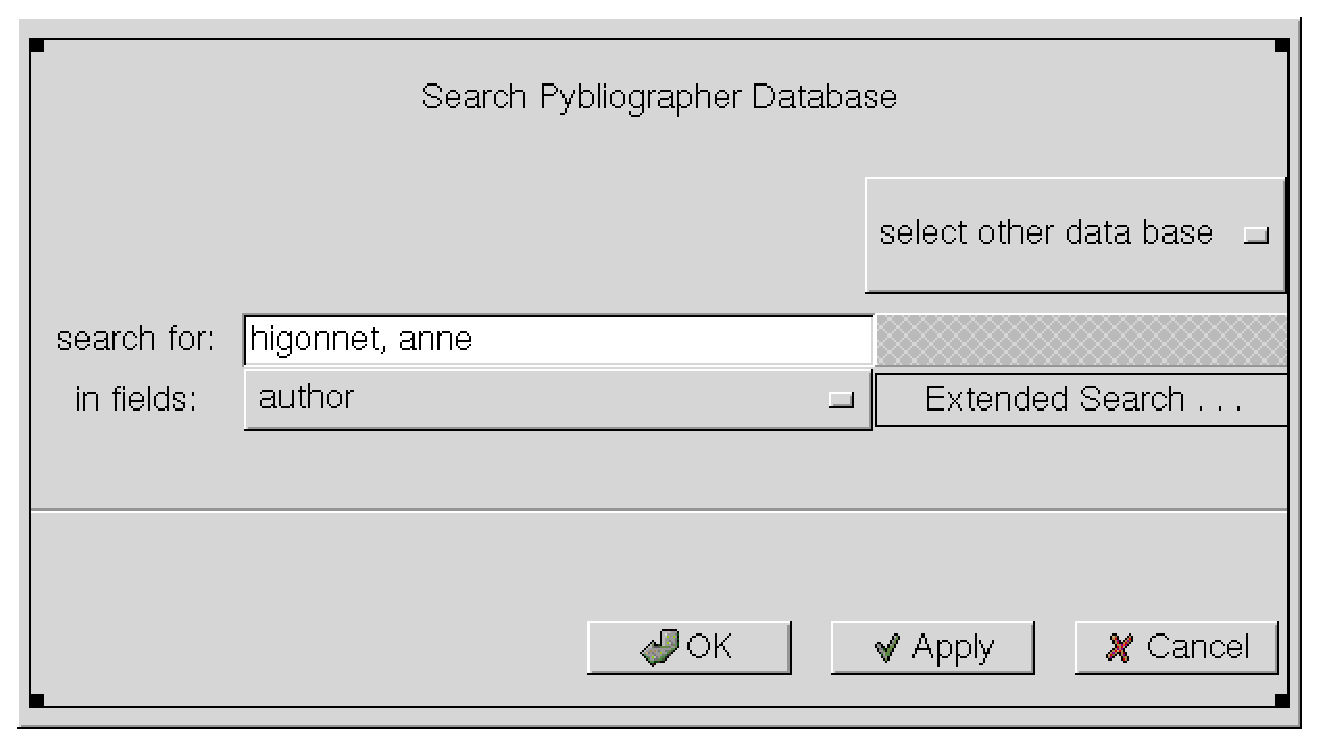
\includegraphics[width=.6\textwidth,bb=0 0 617 342]{pics/searchx1.eps}
  \caption{Search window with example search terms entered.}
  \label{fig:searchx1}
\end{figure}


The system replies by displaying the list of one item found, and also
the first and only item in a subwindow (Fig. \ref{fig:searchx2})

\begin{figure}[h]
  
  \caption{Display of example search results}
  \label{fig:searchx2}
\end{figure}

You decide to e-mail the citation to your friend. You can easily
insert it into the e-mail with the standard \textit{drag-and-drop}
mechanism that Pybliographer supports. The format of the citation is
easily selected and changed (XXX).

Perhaps you should try and look for some other references in this area
when your are in the library again? Let's attach a note to the item,
so as to be reminded of it when you visit the library the next time: 

\begin{figure}[h]
  
  \caption{Adding an action note}
  \label{fig:searchx3}
\end{figure}


\paragraph{Writing an article}

\label{sec:writing-an-article}

It's only a short note this time, so we don't need much preparation. A
review say, the book lays on your table, a couple of notes, the editor
is started. You didn't enter the book into your database yet, so you
start with querying your national library (see Fig.~\ref{fig:searchx4}
). This has the useful side effect of telling you whether the author
in question has already published something (no need to put your foot
in it).

\begin{figure}[h]
  
  \caption{Looking up an author in an external database}
  \label{fig:searchx4}
\end{figure}

Whenever you look something up in this way in an \textit{external
  databaese}, as opposed to the Pybliographer database, the result of
your query will be captured in an internal list, it is then available
for further processing, but not yet entered into the Pybliographer
database. The reason for this is, that it may be too much work for the
moment -- and it is work that must be done diligently -- to check-in
and adapt each an every item that a database query might deliver. (See
the next chapter, in particular ... for more information on this.)
But in this case, there are but two items, which are easily added.

If the information comes, as it is here presumably the case, from a
Z39.50 connected and MARC serving database, there is usually little to
do at this stage. One point, however, remains to do: the new entries
must be correctly categorised, lest our fine arrangement goes to
pieces. If we are content with the standard folder mechanism, it
should suffice to travers the folder hierarchy until the right leave
is found, then to drop the item(s).

\begin{figure}[h]
  
  \caption{Dragging an item into a folder}
  \label{fig:searchx5}
\end{figure}
 
To commence the article, you drag the corresponding item on the editor
window and drop it there: the formatted bibliographical reference is
inserted and easily edited by you for publication.

You follow this first paragraph by your observations, occasionally
consulting your paper notes perhaps. Oh, and this paragraph on page
123 you would like to quote, but first you enter it in Pybliographer's
quotation storage. (XXX) A new editor window appears and already knows
the item from which you want to enter the text. It first asks you for
the page number, so you cannot forget it, and then lets you enter and
edit the text. 

\begin{figure}[h]
  
  \caption{Entering a quotation}
  \label{fig:searchx6}
\end{figure}

By simply dragging the quote into the editor window you not only get
the text, but the citation as well. You decide to use only a portion
of the full quote, so you delete a portion of it. Then you want to add
another voice, whatever was his name \dots\ You decide to open the
author list and position it at the approximate name.

\begin{figure}[h]
  
  \caption{Displaying the author list}
  \label{fig:searchx7}
\end{figure}

You select and open the right entry (let's assume this), and
look down the list until you find the wanted entry. From the detail
view of this entry you could again choose a quote, but then you
decide otherwise, and simply cite this article instead, you already
guess, how to do it.

\begin{figure}[h]
  
  \caption{Citing an item}
  \label{fig:searchx9}
\end{figure}

Let's stay for a moment yet with the detil view: the article had been
quoted, you remember, and selecting the references view lets you find
this article as well. A sentence from here would fit in much better
with you review, wouldn't it? 

\begin{figure}[h]
  
  \caption{Excerpt -- sections and quotes}
  \label{fig:searchxa}
\end{figure}

When you are finished with your work, Pybliographer does the
bibliography for you, simply select Format/references from the
Menu. You need to specify a stylesheet, and some other options, and
then you can lay back and relax.

\begin{figure}[h]
  
  \caption{Dialogue Formatting options}
  \label{fig:dlformat1}
\end{figure}



%%% Local Variables: 
%%% mode: latex
%%% TeX-master: "td-td2"
%%% End: 
